\documentclass[11pt,letterpaper]{article}     % Tipo de documento y otras especificaciones
\usepackage[utf8]{inputenc}                   % Para escribir tildes y eñes
\usepackage[spanish]{babel}                   % Para que los títulos de figuras, tablas y otros estén en español
\usepackage[apaciteclassic]{apacite}
\usepackage{geometry}    
\usepackage{textcomp}
\geometry{left=25mm, right=25mm, top=25mm, bottom=25mm} % Tamaño del área de escritura de la página
\usepackage{amsmath}      % Los paquetes ams son desarrollados por la American Mathematical Society
\usepackage{amsfonts}     % y mejoran la escritura de fórmulas y símbolos matemáticos.
\usepackage{booktabs}
\usepackage{subfig}
\usepackage{amssymb}
\usepackage{graphicx}     % Para insertar gráficas
\usepackage{float}		% Para ubicar las tablas y figuras justo después del texto
\usepackage{pdfpages}
\batchmode
\usepackage{enumerate}
\usepackage{siunitx}
\pagestyle{plain} 
\usepackage{graphics}
\pagenumbering{arabic}
\usepackage{multicol}   % Para varias columnas
\usepackage{multirow}
\usepackage{color}%Paquete para colocar color al texto
%====================Español Venezolano Rápido============================
\renewcommand\tablename{Tabla}
\renewcommand\figurename{Figura}
%\renewcommand\prefacename{Prefacio}
\renewcommand\refname{REFERENCIAS}
%\renewcommand\bibname{REFERENCIAS}
\renewcommand\abstractname{Resumen}
%\renewcommand\chaptername{CAPÍTULO}
\renewcommand\appendixname{Apéndice}
\renewcommand\contentsname{ÍNDICE GENERAL}
\renewcommand\listfigurename{LISTA DE FIGURAS}
\renewcommand\listtablename{LISTA DE TABLAS}
\renewcommand\indexname{Índice Alfabético}
\renewcommand\partname{Parte}

%\renewcommand\enclname{Adjunto}
%\renewcommand\ccname{Copia a}
%\renewcommand\headtoname{A}
%\renewcommand\pagename{Página}
%\renewcommand\seename{véase}
%\renewcommand\alsoname{véase también}
%\renewcommand\proofname{Demostración}
%\renewcommand\glossaryname{Glosario}
%===================  Español venezolano =====================


\author{\\Omaña Enderson CI: 24.757.361\\Raven Guillermo CI: 25.476.227\\Profesor: Crespo Jorge \vspace*{1in}}
\title{Universidad Central de Venezuela\\{ Facultad de Ingeniería\\Escuela de Ingeniería Eléctrica\\ Conversión Electromecánica de la energía\\\vspace*{1.5in} }Laboratorios 6 y 7\\MAQUINAS DE CORRIENTE CONTINUA\vspace*{1.35in}}
\date{Caracas, \today}

\begin{document}	% Inicio del documento
\maketitle							% Título
\newpage
\tableofcontents
\newpage
\section{Objetivos}
\begin{itemize}
	\item Estudiar los diferentes tipos de motores de corriente continua y sus
    aplicaciones en la industria.
	\item Modelar en régimen permanente una máquina de corriente continua.
	\item Determinar las curvas características más importantes de las máquinas de
    corriente continua.
    \item Estudiar los problemas asociados a la conmutación de una máquina de
    corriente continua.
\end{itemize}

\section{Lista de instrumentos}
\begin{table}[H]
	\caption{Lista de instrumentos de medición y componentes}
	\centering
	\begin{tabular}{|c|c|}
		\hline 
		Instrumento & Alcance ó especificaciones \\ \hline 
		Reostato &  (0-100) $\Omega$; 2.4 A \\  
		\hline 
		Reostato &  (0-33) $\Omega$; 4.2 A \\  
		\hline
		Voltímetros de bobina móvil y hierro móvil &  (0-150) V/ (0-15) V/(0-30) V/(0-300) V\\  
		\hline 
			Multímetro fluke & -\\  
		\hline 
		Resistencia de shunt & 40 A @ 60 mV\\  
		\hline
		Tacometro & -\\  
		\hline
		Amperímetro de bobina móvil y hierro móvil &(0-1.2) A/ (0-6) A/(0-30) A \\ 
		\hline
		Protecciones AC & 25 A; 380 V\\ 
		\hline
		Protecciones DC & -\\ 
		\hline
		Carga lineal & (200,400,600,800,1K)W  \\
        \hline
        \multirow{8}{3cm}{Motor sincrónico} & 3.5 KVA \\ 
        \cline{2-2}
        & 120/208 V \\
        \cline{2-2}
        & 16,8/9,7 A\\
        \cline{2-2}
        &1000 rpm\\
        \cline{2-2}
        &Iexc 3 A\\
        \cline{2-2}
        &Vexc 125 V\\
        \cline{2-2}
        & fp 0,9
        \\ \hline
        \multirow{5}{3cm}{Motor DC} & 115 V \\ 
        \cline{2-2}
        & 56A  \\
        \cline{2-2}
        & 1000 rpm\\
        \cline{2-2}
        &6,5 hp\\
        \cline{2-2}
        &carga 100\%\\
        \hline
        \multirow{5}{3cm}{Generador DC} & 3 KV\\ 
        \cline{2-2}
        & 125 V \\
        \cline{2-2}
        &26,5 A\\
        \cline{2-2}
        & 1000 rpm\\
        \hline

        
	\end{tabular} 
\end{table}
\section{Condiciones de ensayo}
Estas son las precauciones y normativas necesarias para realizar el laboratorio de forma segura y efectiva: 
\begin{itemize}
    \item \textbf{Respecto a la medición de la curva en vacío:} La máquina a la que se le hará la prueba deberá estar conectada como generador. Dado que tiene que girar a velocidad constante, se utilizara algún mecanismo externo que brinde tales características. 
    
    Este sera un motor sincrónico o una turbina. En el caso de emplearse un motor sincrónico el campo deberá activarse al alcanzar una velocidad constante.
    \item \textbf{Respecto a la medición de resistencias:} Se trabajara asegurándose que la corriente máxima alcanzada en $I_{f}$ ó $I_{a}$ sea menor o igual al 10 \% de la corriente nominal. La resistencia obtenida mediante la pendiente de la recta debe ajustarse de acuerdo a la temperatura.
    \item \textbf{Respecto a la medición de la característica de regulación:} Se debe mantener $U_{c}$ (tensión en los bornes) en su valor nominal y a velocidad nominal. 
    \item  \textbf{Respecto a la medición del porcentaje de regulación:} Se debe comenzar a medir la tensión en los bornes comenzando desde el valor a plena carga.
    \item \textbf{Respecto a la medición de la curva de carga:} Se debe medir a velocidad constante.
    \item \textbf{Respecto a la medición de la curva electromecánica de par:} Se deben mantener $U_{c}$ constante y $I_{exc}$.
    \item \textbf{Respecto a la medición de la curva electromecánica de velocidad:} La tensión en los bornes (Uc) deberá mantenerse a su valor nominal y la corriente de excitación también.
    \item  \textbf{Respecto a la medición del porcentaje de regulación de velocidad:} Se comenzara a medir desde la carga nominal ($I_{a}$ nominal y N nominal).
    \item  \textbf{Respecto a la medición de la curva de regulación de velocidad:} Sin importar si se utiliza el método de control por corriente de campo ó el método de ajuste de tensión en los terminales de armadura. Es necesario mantener en ambos el par constante, aunque en el primero la corriente de excitación es constante, en cambio en el segundo sera constante la tensión en los bornes.
    \item  \textbf{Respecto a la medición de la curva de regulación de par:} Sin importar si se utiliza el método de control por corriente de campo ó el método de ajuste de tensión en los terminales de armadura. Es necesario mantener en ambos la velocidad constante, aunque en el primero la corriente de excitación es constante, en cambio en el segundo sera constante la tensión en los bornes.  
    \item \textbf{Respecto a la  vestimenta:} No usar franelas o camisas manga larga, llevar zapatos de goma y pantalones. No usar collares ni pulseras de metal.
    \item \textbf{Previo a las pruebas:} Hacer primero el montaje antes de energizar, al culminarlo preguntar al profesor si las conexiones son correctas para proceder con las pruebas.
    \item \textbf{Respecto a la comunicación:} Mantener informado sobre cualquier cambio en el montaje al compañero de laboratorio y por sobre todo informar si el circuito se encuentra energizado o no.
	\item \textbf{Respecto a las curvas observadas:} No aceptar como adecuada una curva que este llena de ruido, ya que se puede deber a que algún elemento puede estar actuando como antena, esto originara incertidumbre en los resultados.
	\item \textbf{Respecto al numero de mediciones:}
	Realizar al menos 5 mediciones para condiciones distintas.
	\item \textbf{Respecto a la elección de componentes y las conexiones:} Evitar los componentes que puedan funcionar como antenas (como resistencias de shunt de tipo mariposa u algún otro que se encuentre muy expuesto) y cuidar los contactos de cada conexión.
    \item \textbf{Respecto a la manipulación:} En caso de maniobrar el circuito energizado manipular con la mano derecha, buscando mayores probabilidades de sobrevivir en caso de un accidente eléctrico.
\end{itemize}
\section{Procedimiento}
\subsection{Características internas}
\subsubsection{Caídas internas}
\begin{enumerate}
    \item Lo primero sera, hallar las resistencias internas de campo y armadura por lo que se realizaran las conexiones como en la Figura \ref{fig:diagMedRes}.
    \item Se conectara unicamente el lado de campo con una fuente DC (a una fracción del valor nominal).
    \item Manteniendo la tensión $V_{f}$ fija y variando el reostato en pasos equidistantes se tomara nota de los valores de tensión y corriente. Se tomaran al menos 4 mediciones.
    \item Se desconectara la alimentación del lado de campo y se conectara la fuente del lado serie repitiendo así los pasos previos.
    \item Se desconectara la alimentación del lado serie y se conectara la fuente del lado de armadura a tensión por debajo del valor nominal.
    \item Manteniendo la tensión $V_{a}$ fija y desplazando la cuchilla de arranque en pasos equidistantes se tomara nota de los valores de tensión en los bornes y la tensión en la resistencia de shunt. Se tomaran al menos 5 mediciones.
    
    \item Se desconectara la alimentación del lado de armadura y se des-energizara el circuito.
\end{enumerate}
\subsubsection{Curva de saturación ó vacío}
\begin{enumerate}
	\item Se armara el esquema de conexiones conectando el motor DC como generador de acuerdo a la figura \ref{fig:diagMedCurvaCaracteristica}.
	\item Se encenderá el generador sincrónico y solo cuando alcance una velocidad constante se accionara el campo mediante las protecciones DC.
	\item Manteniendo la velocidad del eje a su valor nominal se variara el reostato del lado de campo de forma que los datos sean tomados en espacios apropiados que permitirán una exactitud de la curva graficada entre nula excitación y 125 \% de la tensión nominal ($U_{nom}$), en la parte lineal de la curva con incrementos de 20 \% de $U_{nom}$ y pasos del 10 \% de $U_{nom}$,
	alrededor del codo de saturación que suele estar entre el 80 \% y el 110 \% de la $U_{nom}$.  
	\item Se repetirá el proceso del punto previo; pero desde el ultimo punto alcanzado hasta el valor mínimo, respetando en lo posible que los pasos sean iguales.
\end{enumerate}
\subsection{Características externas}
\subsubsection{Característica de regulación y porcentaje de regulación}
\begin{enumerate}
    \item Se realiza la conexión de la Figura \ref{fig:diagGeneradorIndependiente} de generador independiente.
    \item Empleando el tacómetro se verifica velocidad nominal en el generador.
    \item Se ajusta $U_{c}$ inicialmente sin carga hasta alcanzar $U_{nom}$ con $I_{ext}$, una vez alcanzado $U_{nom}$ se registra el valor.
    \item Se conecta carga al sistema, generando un cambio en los valores de $U_{c}$ e $I_a$.
    \item Se ajusta $U_{c}$ con $I_{ext}$ hasta alcanzar valores nominales. Se registra el valor de $I_{ext}$ e $I_a$.
    \item Se varía la carga y se repite hasta llegar a valores nominales.
    \item Una vez registrado el ultimo valor se verifica que se encuentre en $U_{nom}$ e $I_{anom}$ en caso que sean diferentes se ajustarán a valores nominales, una vez verificado se desconectará la carga de forma gradual hasta retirarla completamente, luego se registra e valor de $U$ sin carga. 
\end{enumerate}
\subsection{Motor independiente}
\subsubsection{Curva de velocidad en función de la corriente de armadura}
\begin{enumerate}
    \item Se realiza la conexión de la fig \ref{fig:diagMotorIndependiente} de motor independiente.
    \item Se realiza la medición de la curva electromecánica de velocidad manteniendo Uc constante e $I_{ext}$ constante.
    \item Se anotan las mediciones de $I_a$ y de la velocidad.
    \item Se varia Rs, por lo que varia $I_a$ directamente. Se anotan los valores y se repite hasta tener varias mediciones.
\end{enumerate}
\subsubsection{Determinar el PRN\%}
\begin{enumerate}
    \item Se toman las medidas a $I_a$ nominal y N nominal con tensión de armadura e Iexc constante.
    \item Se eleva la carga lineal hasta el valor nominal del motor. Se registran los datos
    \item Se quita la carga y se toman los datos.
\end{enumerate}
\subsection{Pérdidas en vacío}
\begin{enumerate}
    \item Para calcular las perdidas en el vacío se deben realizar medidas en dos velocidades distintas anotando los valores de corriente y tensión asociados.
\end{enumerate}
\section{Diagramas}
\begin{figure}[H]
    \centering
    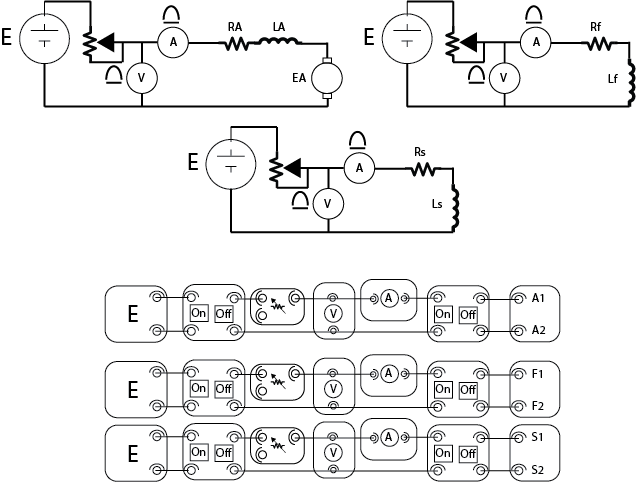
\includegraphics[scale=0.5]{./recursos-Lab6/diagMedRes.png}
    \caption{Diagrama de conexión pruebas de resistencias internas}
    \label{fig:diagMedRes}
\end{figure}
\begin{figure}[H]
    \centering
    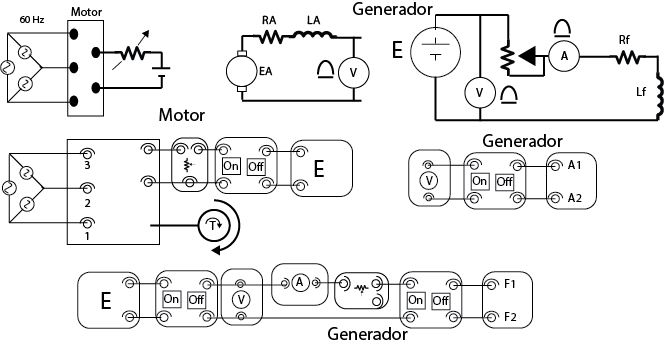
\includegraphics[scale=0.5]{./recursos-Lab6/diagMedCurvaVacio.png}
    \caption{Diagrama de conexión pruebas de Prueba curva de vacio}
    \label{fig:diagMedCurvaCaracteristica}
\end{figure}
\begin{figure}[H]
    \centering
    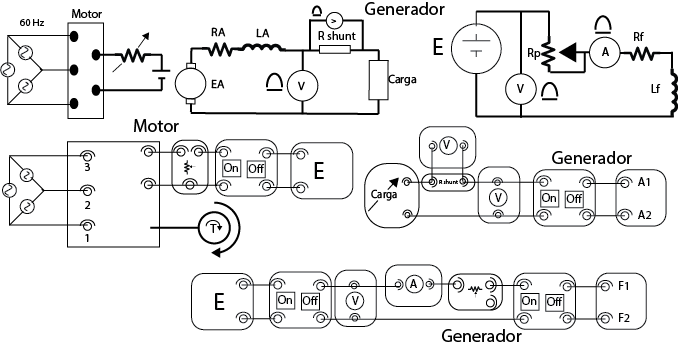
\includegraphics[scale=0.5]{./recursos-Lab6/diagGeneradorIndependiente.png}
    \caption{Diagrama de conexión de generador independiente}
    \label{fig:diagGeneradorIndependiente}
\end{figure}
\begin{figure}[H]
    \centering
    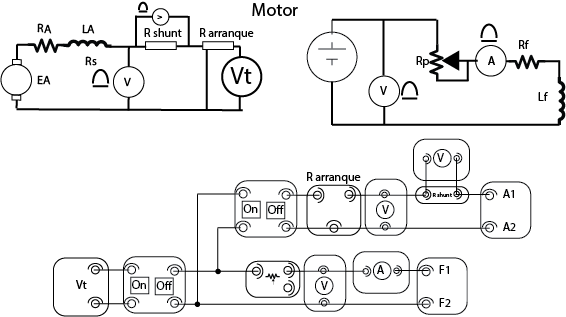
\includegraphics[scale=0.5]{./recursos-Lab6/diagMotorIndependient.png}
    \caption{Diagrama de conexión de motor independiente}
    \label{fig:diagMotorIndependiente}
\end{figure}
\section{Cálculos preliminares}
\subsection{Características internas}
\subsubsection{Resistencia interna }
De acuerdo al diagrama de la figura \ref{fig:diagMedRes}, se espera una curva característica de tensión vs corriente para el lado de campo con una forma similar al de la figura \ref{fig:curvaCaractPreVILadoCampo} y en el lado de armadura su forma se asemejara a la figura \ref{fig:curvaCaractPreVILadoArmadura}.
\begin{figure}[H]
    \centering
    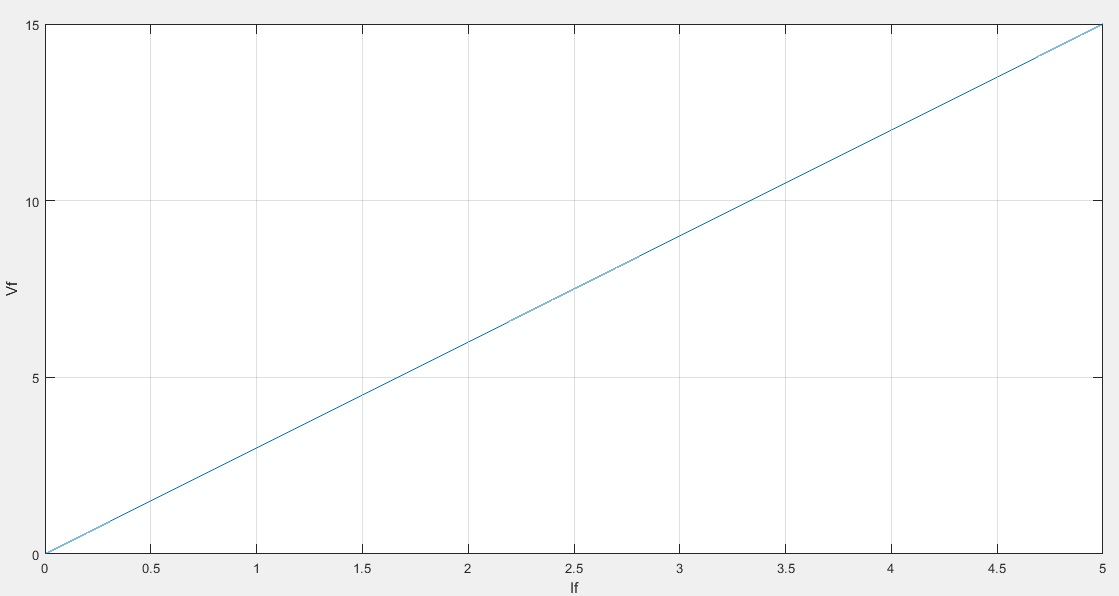
\includegraphics[scale=0.5]{./recursos-Lab6/curvaCaractPreVILadoCampo.jpg}
    \caption{Curva característica esperada V vs $I_{f}$}
    \label{fig:curvaCaractPreVILadoCampo}
\end{figure}
La pendiente de la curva previa proporcionara el valor de la resistencia de campo.
\begin{figure}[H]
    \centering
    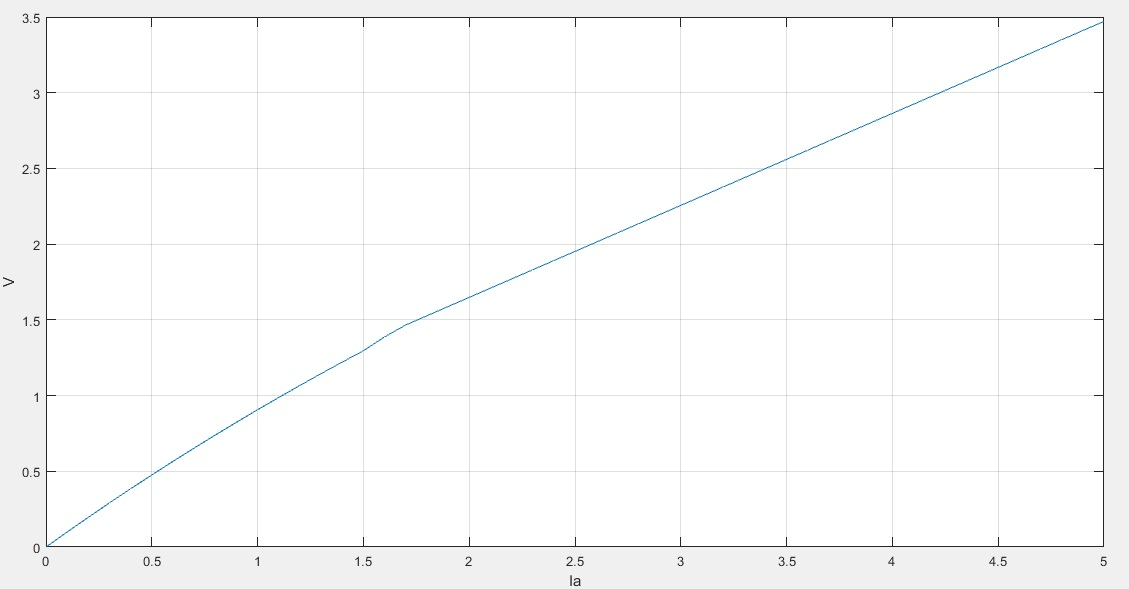
\includegraphics[scale=0.5]{./recursos-Lab6/curvaCaractPreVILadoArmadura.jpg}
    \caption{Curva característica esperada V vs $I_{a}$}
    \label{fig:curvaCaractPreVILadoArmadura}
\end{figure} 
Como se puede observar en la figura \ref{fig:curvaCaractPreVILadoArmadura} a diferencia de la figura \ref{fig:curvaCaractPreVILadoCampo} no es una recta completamente. Al inicio de la curva se espera un comportamiento no lineal debido a la resistencia de las escobillas; Aunque desde cierto punto se vuelve lineal debido a que el ya mencionado efecto es despreciable, por lo que la pendiente de la zona lineal corresponde con el valor de la resistencia de armadura. 
\section{Resultados}
\subsection{Características internas}
\subsubsection{Resistencia de campo}
Se realizaron las siguientes mediciones:
\begin{table}[H]
	\centering
	\caption{Valores obtenidos por método de voltímetro-amperímetro para Rf}
	\label{VoltimetroAmperimetroRf}
	\begin{tabular}{|c|c|}
		\hline
		\textbf{Tensión {[}V{]}} & \textbf{Corriente {[}A{]}} \\ \hline
		6,0 $\pm$ 0,1            & 0,12 $\pm$ 0,02            \\ \hline
		7,0 $\pm$ 0,1            & 0,14 $\pm$ 0,02            \\ \hline
		8,0 $\pm$ 0,1            & 0,16 $\pm$ 0,02            \\ \hline
		8,5 $\pm$ 0,1            & 0,18 $\pm$ 0,02            \\ \hline
		9,0 $\pm$ 0,1            & 0,2 $\pm$ 0,02             \\ \hline
	\end{tabular}
\end{table}
Utilizando los valores del cuadro \ref{VoltimetroAmperimetroRf} se linealizo mediante mínimos cuadrados y se obtuvo lo siguiente:
\begin{figure}[H]
	\centering
	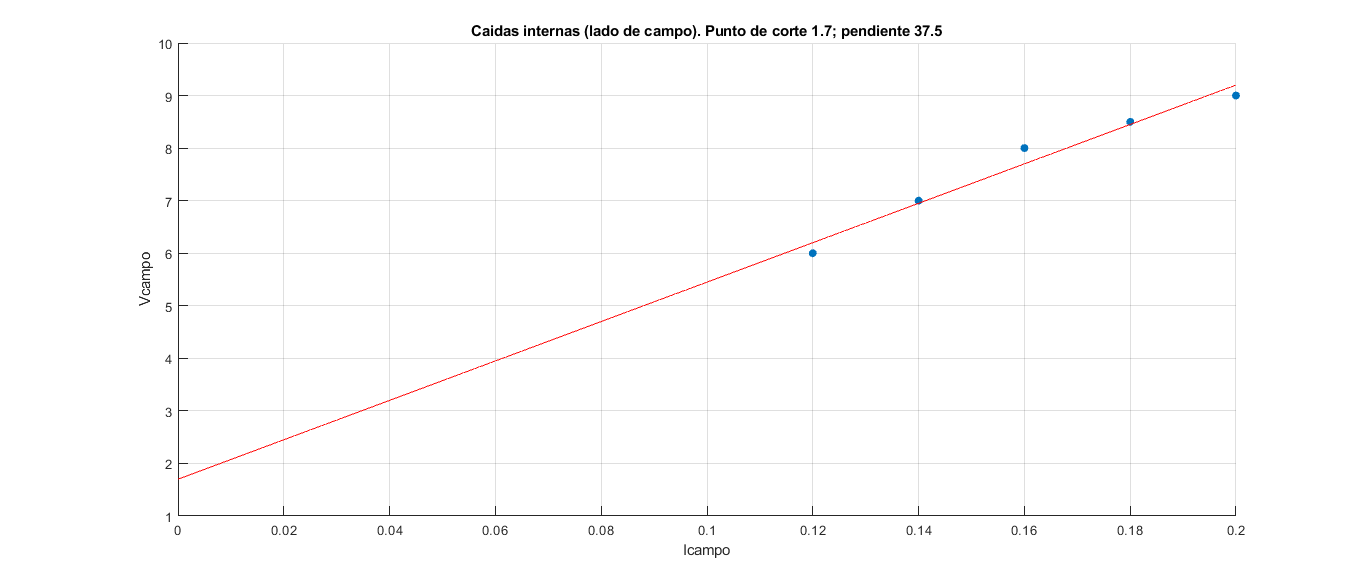
\includegraphics[scale=0.5]{./recursos-Lab6/caidasInternasCAMPO.png}
	\caption{Recta obtenida por regresión lineal que corresponde con la resistencia de campo}
	\label{fig:rectaResistenciaCampo}
\end{figure}
Para calcular la incertidumbre asociada a la pendiente hallada se determino la desviación estándar:
\begin{equation}
	\sigma = \sqrt{\frac{\sum_{i=1}^{N}(y_{i}-m\cdot x_{i}-b)^{2}}{N-2}} \label{desvEstandar}
\end{equation}
Donde:\\
N: numero de datos\\
b: Punto de corte obtenido\\
m: Pendiente obtenida\\
$y_{i}$: Datos del eje y\\
$x_{i}$: Datos del eje x

Utilizando la desviación se calcula incertidumbre de la pendiente mediante la siguiente ecuación:
\begin{equation}
	\Delta m = \sigma \sqrt{\frac{N}{N\sum_{i=1}^{N}x_{i}^{2}-\left(\sum_{i=1}^{N}x_{i}\right)^{2}}} \label{incertiPendiente}
\end{equation}
Por lo tanto la resistencia de campo medida sera: $R_{f(medida)}$ = 37,50 $\pm$ 0,29 $\Omega$. No obstante se requiere ajustar el valor respecto a la temperatura empleando la siguiente expresión:
\begin{align}
	R_{f} = R_{(medida)} \frac{T_{r}+T_{k}}{T_{m}+T_{k}} \label{ajusteTemp}
\end{align}
donde:\\
$T_{k}$ : 234.5 \textdegree C (cobre).\\
$T_{m}$ : Temperatura a la cual se midió la resistencia, 25 \textdegree C.\\
$T_{r}$ : Es la temperatura de referencia en \textdegree C (75 \textdegree C).\\
Entonces: $R_{f(ajustada)}$ = 44,73 $\pm$ 0,29 $\Omega$.
\subsubsection{Resistencia de armadura y tensión en escobillas}
Se realizaron las siguientes mediciones:
\begin{table}[H]
	\centering
	\caption{Valores obtenidos por método de voltímetro-amperímetro para Ra}
	\label{VoltimetroAmperimetroRA}
	\begin{tabular}{|c|c|}
		\hline
		\textbf{Tensión {[}V{]}} & \textbf{Corriente {[}A{]}} \\ \hline
		0,869 $\pm$ 0,001            & 2,5 $\pm$ 0,5            \\ \hline
		1,356 $\pm$ 0,001            & 4,0 $\pm$ 0,5            \\ \hline
		1,563 $\pm$ 0,001            & 5,0 $\pm$ 0,5            \\ \hline
		1,751 $\pm$ 0,001            & 5,5 $\pm$ 0,5            \\ \hline
		2,220 $\pm$ 0,001            & 7,5 $\pm$ 0,5             \\ \hline
		2,737 $\pm$ 0,001            & 10,0 $\pm$ 0,5             \\ \hline
	\end{tabular}
\end{table}
Empleando los valores del cuadro \ref{VoltimetroAmperimetroRA} se linealizo mediante mínimos cuadrados y se obtuvo lo siguiente:
\begin{figure}[H]
	\centering
	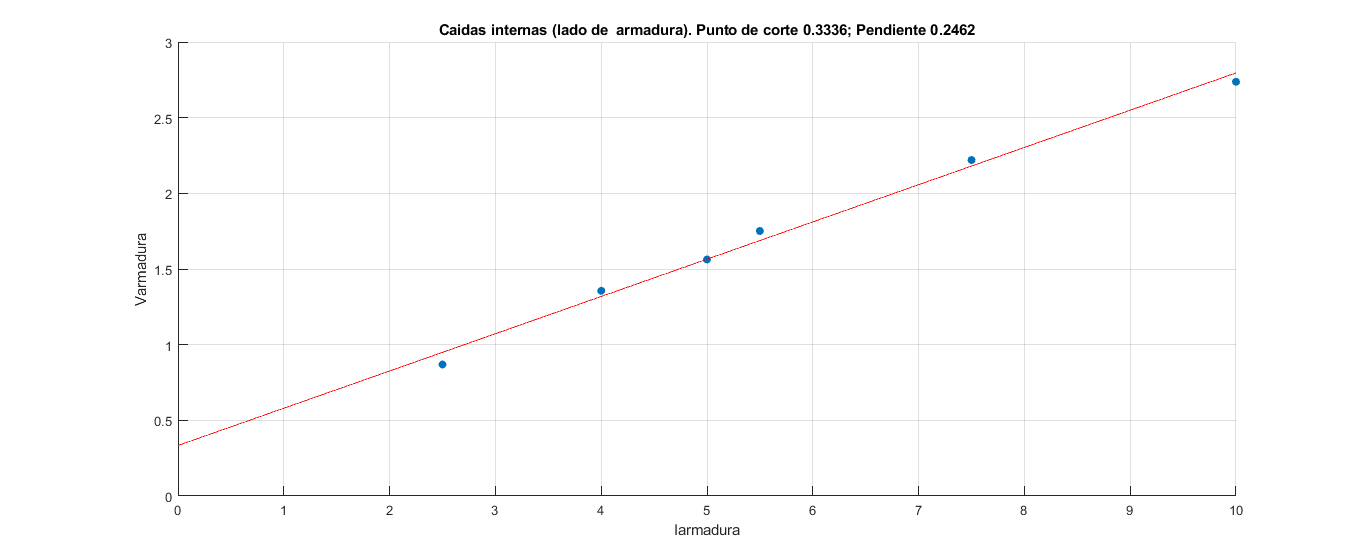
\includegraphics[scale=0.5]{./recursos-Lab6/caidasInternasARMADURA.png}
	\caption{Recta obtenida por regresión lineal que corresponde con la resistencia de armadura y tensión en escobillas}
	\label{fig:rectaResistenciaArmadura}
\end{figure}
Utilizando los datos obtenidos de la recta que corresponden con la resistencia de armadura y las ecuaciones \ref{desvEstandar} y \ref{incertiPendiente} se obtuvo que la resistencia de armadura medida es igual a: $R_{a(medida)}$ = = 0,2462 $\pm$ 0,0081 $\Omega$. No obstante se requiere ajustar el valor respecto a la temperatura usando la ecuación \ref{ajusteTemp}, de esta forma la resistencia de armadura real sera: $R_{a(ajustada)}$ = 0,2936 $\pm$ 0,0081 $\Omega$.

Por otro lado la tensión en las escobillas corresponde con el punto de corte con el eje y, la incertidumbre del mismo se calcula con:
\begin{equation}
	\Delta V_{esc} = \sigma \sqrt{\frac{\sum_{i=1}^{N}x_{i}^{2}}{N\sum_{i=1}^{N}x_{i}^{2}-\left(\sum_{i=1}^{N}x_{i}\right)^{2}}}
\end{equation}
Entonces dicha tensión sera: $V_{esc}$ = 0,3336 $\pm$ 0,0195 V. De acuerdo con IEC 34-2 e IEEE Std 113-1985 las escobillas del motor deben ser del tipo metal-grafito, con shunt debido a su tensión reducida. 
\subsubsection{Modelo Obtenido}
%% Enderson haz un diagrama circuital con conexión independiente donde le coloques el valor de las resistencias obtenidas con sus incertidumbres y la tensión en las escobillas obtenida
\begin{figure}[H]
	\centering
	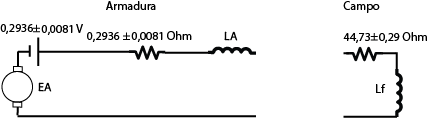
\includegraphics[scale=0.9]{./recursos-Lab6/diagModeloObtenido.png}
	\caption{Modelo que incluye valores obtenidos}
	\label{fig:modObtenido}
\end{figure}
\subsubsection{Resistencia serie}
Se realizaron las siguientes mediciones:
\begin{table}[H]
	\centering
	\caption{Valores obtenidos por método de voltímetro-amperímetro para Rs}
	\label{VoltimetroAmperimetroRs}
	\begin{tabular}{|c|c|}
		\hline
		\textbf{Tensión {[}mV{]}} & \textbf{Corriente {[}A{]}} \\ \hline
		7,3 $\pm$ 0,1            & 0,44 $\pm$ 0,02            \\ \hline
		8,5 $\pm$ 0,1            & 0,52 $\pm$ 0,02            \\ \hline
		9,0 $\pm$ 0,1            & 0,54 $\pm$ 0,02            \\ \hline
		10,0 $\pm$ 0,1            & 0,60 $\pm$ 0,02            \\ \hline
		11,4 $\pm$ 0,1            & 0,70 $\pm$ 0,02             \\ \hline
		13,6 $\pm$ 0,1            & 1,00 $\pm$ 0,02             \\ \hline
	\end{tabular}
\end{table}
Utilizando los valores del cuadro \ref{VoltimetroAmperimetroRs} se linealizo mediante mínimos cuadrados y se obtuvo lo siguiente:
\begin{figure}[H]
	\centering
	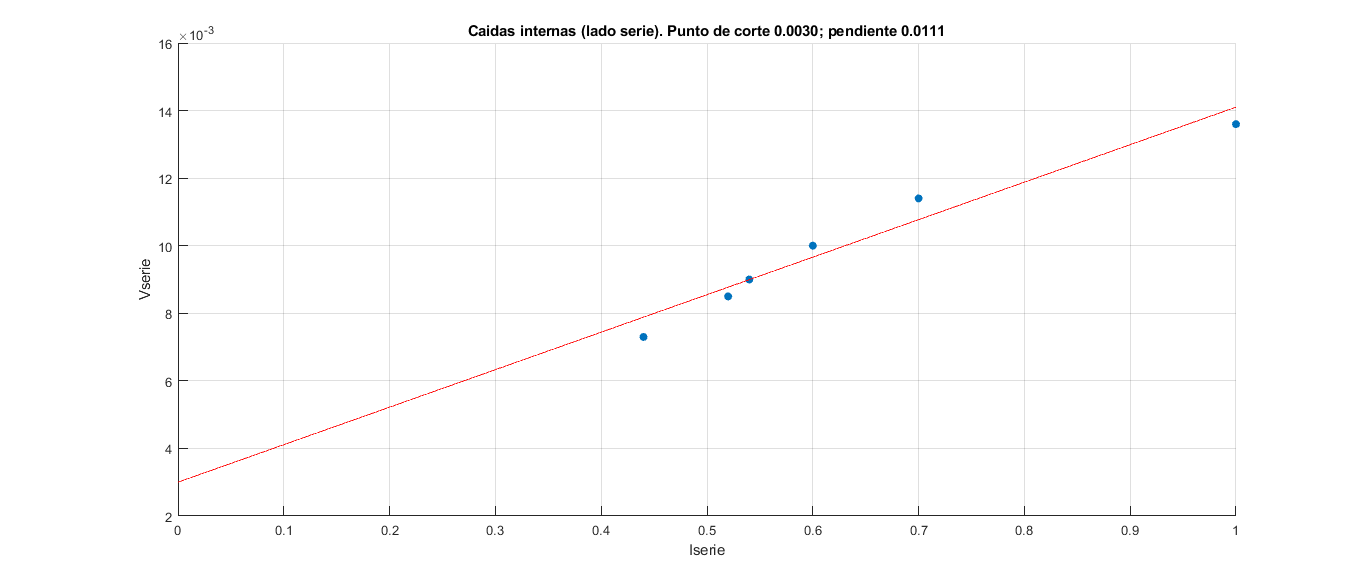
\includegraphics[scale=0.5]{./recursos-Lab6/caidasInternasSERIE.png}
	\caption{Recta obtenida por regresión lineal que corresponde con la resistencia serie}
	\label{fig:rectaResistenciaSerie}
\end{figure}
Empleando los datos obtenidos de la recta que corresponden con la resistencia serie y las ecuaciones \ref{desvEstandar} y \ref{incertiPendiente} se obtuvo que la resistencia en serie es igual a: $R_{s}$ = 11,05 $\pm$ 0,35 m$\Omega$.  No obstante se requiere ajustar el valor respecto a la temperatura usando la ecuación \ref{ajusteTemp}, de esta forma la resistencia serie real sera: $R_{s(ajustada)}$ = 13,18 $\pm$ 0,35 m$\Omega$.
\subsubsection{Curva de vacío}
Se realizaron mediciones de corriente y tensión a una velocidad constante de 1140 $\pm$ 2 rpm.
\begin{table}[H]
	\centering
	\caption{Mediciones de tensión de vacío y corriente de campo}
	\label{MedCurvaVacio}
	\begin{tabular}{|c|c|c|c|}
		\hline
		\multicolumn{2}{|c|}{Elevando}                        & \multicolumn{2}{c|}{Reduciendo}                       \\ \hline
		\textbf{$U_{0}$ {[}V{]}} & \textbf{$I_{exc}$ {[}A{]}} & \textbf{$U_{0}$ {[}V{]}} & \textbf{$I_{exc}$ {[}A{]}} \\ \hline
		60 $\pm$ 1               & 0,54 $\pm$ 0,02            & 109 $\pm$ 1              & 0,8 $\pm$ 0,1              \\ \hline
		74 $\pm$ 1               & 0,66 $\pm$ 0,02            & 90 $\pm$ 1               & 0,7 $\pm$ 0,1              \\ \hline
		89 $\pm$ 1               & 0,82 $\pm$ 0,02            & 80 $\pm$ 1               & 0,62 $\pm$ 0,02            \\ \hline
		107 $\pm$ 1              & 1,00 $\pm$ 0,02            & 73 $\pm$ 1               & 0,54 $\pm$ 0,02            \\ \hline
		132 $\pm$ 1              & 1,3 $\pm$ 0,1              & -                        & -                          \\ \hline
	\end{tabular}
\end{table}
Con los valores obtenidos en el cuadro \ref{MedCurvaVacio} se empleo la función polyfit(x,y,n) (n es el orden del polinomio) de Matlab con el fin de obtener un polinomio que se ajuste a los datos. Y se evaluó el polinomio mediante polyval(), para posteriormente obtener las siguientes curvas:
\begin{figure}[H]
	\centering
	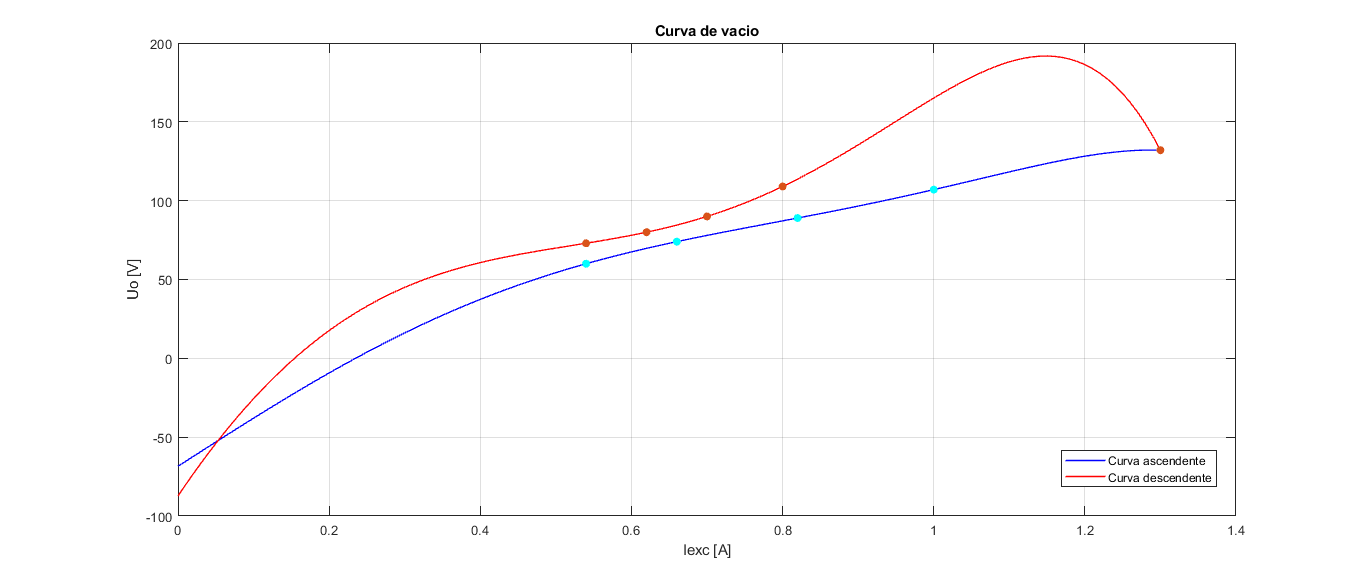
\includegraphics[scale=0.5]{./recursos-Lab6/curvaDeVacioExp.png}
	\caption{Curvas de vacío experimentales}
	\label{fig:curvaDeVacioExp}
\end{figure}
\subsection{Características externas (Funcionamiento como generador)}
\subsubsection{Curva característica de regulación}
Se agrego carga al generador y se ajusto el reostato del lado de campo, con el fin de mantener la velocidad nominal. Se obtuvieron los siguientes resultados:
\begin{table}[H]
	\centering
	\caption{Mediciones del efecto de la carga en la corriente de excitación}
	\label{MedCurvaCaractReg}
	\begin{tabular}{|c|c|}
		\hline
		\multicolumn{2}{|c|}{\textbf{$N_{nominal}$ = 1000 $\pm$ 2 {[}rpm{]}}} \\ \hline
		\textbf{$I_{exc}$ {[}A{]}}   & \textbf{$I_{a}$ {[}A{]}}               \\ \hline
		1,2 $\pm$ 0,1                & 0 (sin carga)                          \\ \hline
		1,3 $\pm$ 0,1                & 8,0 $\pm$ 0,5                          \\ \hline
		1,3 $\pm$ 0,1                & 16,0 $\pm$ 0,5                         \\ \hline
		1,1 $\pm$ 0,1                & 3,5 $\pm$ 0,5 (disminuyendo la carga)  \\ \hline
	\end{tabular}
\end{table}
Utilizando los datos obtenidos en el cuadro \ref{MedCurvaCaractReg}, a excepción punto obtenido al disminuir la carga es posible hallar un polinomio que se ajuste a los datos mediante matlab. En la Figura \ref{fig:curvaCaractReg} se observa el comportamiento del campo respecto a distintas cargas.
\begin{figure}[H]
	\centering
	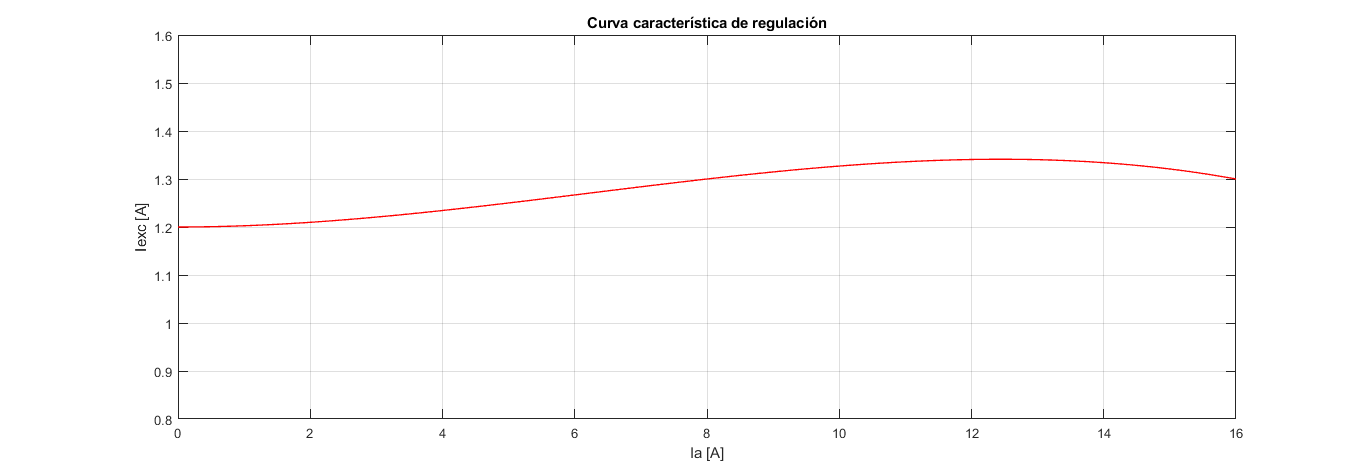
\includegraphics[scale=0.5]{./recursos-Lab6/curvaCaractRegulacion.png}
	\caption{Curvas característica de regulación experimental}
	\label{fig:curvaCaractReg}
\end{figure}
\begin{itemize}
	\item \textbf{Predeterminación de curva característica de regulación}
\end{itemize}
Para determinar la curva teórica se requiere asumir lo siguiente:
\begin{itemize}
	\item $I_{exc,0}$: corresponde con la corriente de campo en vacío obtenida en el cuadro \ref{MedCurvaCaractReg}, siendo 1,2 A.
	\item $E_{n}$: es la tensión nominal de la placa (125 V).
	\item $R_{a}$: se utilizara la obtenida de forma experimental (0,2936 $\Omega$).
	\item $N_{f}$: es el numero de vueltas del embobinado de campo, se asumirá arbitrariamente 1000 vueltas dado que es un valor promedio.
	\item $E_{0}$: es la tensión de vacío asociada a la corriente de excitación en vacío ($I_{exc,0}$), partiendo de la curva ascendente de vacío se obtiene 128,2 V.
\end{itemize}
Bajo dichas condiciones las ecuaciones que rigen el comportamiento de $I_{exc}$ son:
\begin{align}
	N_{f}I_{exc} = N_{f}I_{exc,0} - h \label{IexcRespectoRA}\\
	h = E_{0}-E_{n}-I_{a}R_{a}\label{ReacArm}
\end{align}
Sustituyendo la ecuación \ref{ReacArm} en \ref{IexcRespectoRA} y despejando $I_{exc}$, se tiene:
\begin{equation}
	I_{exc} = I_{exc,0} - \frac{E_{0}-E_{n}-I_{a}R_{a}}{N_{f}}\label{IexcCalculada}
\end{equation}
Empleando la ecuación previa y asumiendo $I_{a}$ iguales a los obtenidos experimentalmente, se obtiene el siguiente cuadro:
\begin{table}[H]
	\centering
	\caption{Calculo de parámetros de la curva característica de regulación y reacción del inducido}
	\label{predeterCaractReg}
	\begin{tabular}{|c|c|c|}
		\hline
		\textbf{$I_{exc}$ {[}A{]}} & \textbf{$I_{a}$ {[}A{]}} & \textbf{h {[}$A\cdot v${]}} \\ \hline
		1,2                        & 0                        & 0                           \\ \hline
		1,1991                     & 8                        & 0,8512                      \\ \hline
		1,2015                     & 16                       & -1,4976                     \\ \hline
		1,1978                     & 3,5                      & 2,1724                      \\ \hline
	\end{tabular}
\end{table}
Utilizando los datos del cuadro previo y los datos experimentales se compara lo calculado con lo experimental en la siguiente Figura:
\begin{figure}[H]
	\centering
	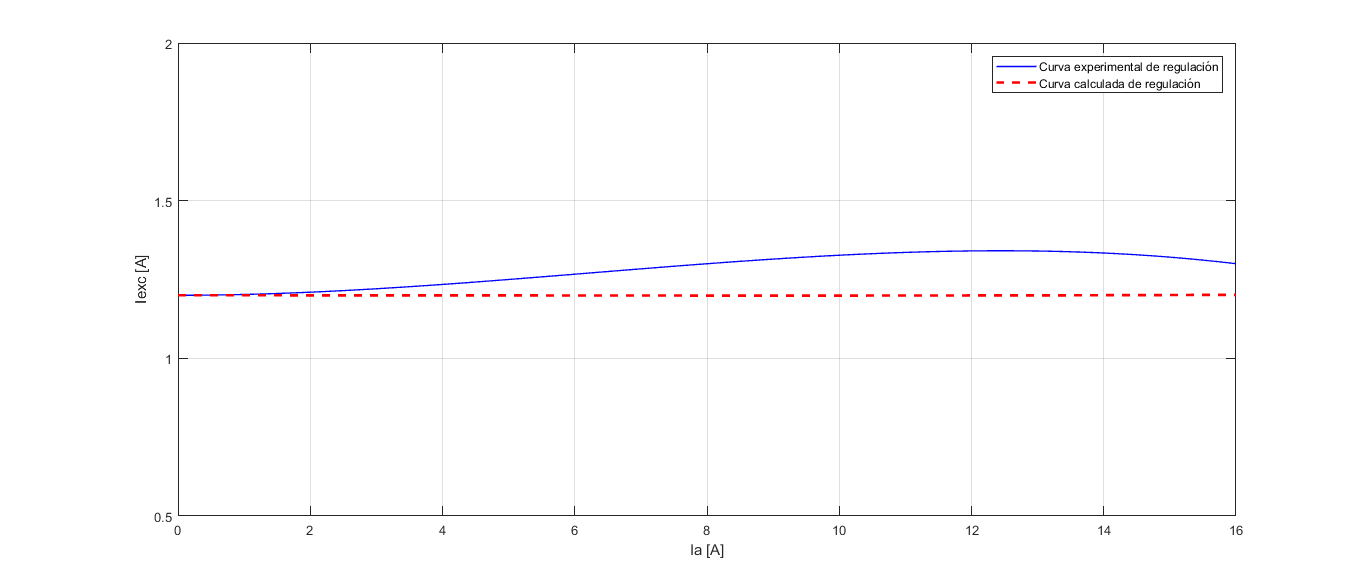
\includegraphics[scale=0.5]{./recursos-Lab6/curvaCaractRegulacionComparacion.png}
	\caption{Comparación de curvas de regulación}
	\label{fig:curvaDeRegComparacion}
\end{figure}
\subsubsection{Porcentaje de regulación}
Se midió la tensión a plena carga y luego sin carga. Se obtuvieron los siguientes resultados:
\begin{table}[H]
	\centering
	\caption{Mediciones para el porcentaje de regulación}
	\label{MedPReg}
	\begin{tabular}{|c|c|}
		\hline
		\textbf{$U_{pc}$ {[}V{]}} & \textbf{$U_{sc}$ {[}V{]}} \\ \hline
		125 $\pm$ 1               & 132 $\pm$ 1               \\ \hline
	\end{tabular}
\end{table}
Se sabe que el porcentaje de regulación de un generador DC viene dado por:
\begin{align}
	\%Reg = \frac{V_{sc}-V_{pc}}{V_{pc}}100\%\\
	\Delta \%Reg = \frac{100}{V_{pc}}\Delta V_{sc} + \frac{V_{sc}}{V_ {pc}^{2}}\Delta V_{pc}
\end{align}
Por medio de las dos ecuaciones previas se obtiene que la regulación es: \%Reg = 5.6 $\pm$ 0.8
\subsubsection{Curva de carga}
Se midió la capacidad del generador para mantener la tensión nominal a distintas cargas (Ver cuadro \ref{MedCurvaCarga}). 
\begin{table}[H]
	\centering
	\caption{Mediciones del efecto de carga en la tensión del generador}
	\label{MedCurvaCarga}
	\begin{tabular}{|c|c|}
		\hline
		\multicolumn{2}{|c|}{\textbf{$U_{c}$ =$U_{nominal}$ = 124 $\pm$ 1}} \\ \hline
		\textbf{$U_{c}$ {[}V{]}}         & \textbf{$I_{a}$ {[}A{]}}         \\ \hline
		120 $\pm$ 1                      & 3,0 $\pm$ 0,5                    \\ \hline
		119 $\pm$ 1                      & 7,5 $\pm$ 0,5                    \\ \hline
		118$\pm$ 1                       & 11,0 $\pm$ 0,5                   \\ \hline
		117$\pm$ 1                       & 15,0 $\pm$ 0,5                   \\ \hline
		116 $\pm$ 1                      & 18,0 $\pm$ 0,5                   \\ \hline
	\end{tabular}
\end{table}
Con los datos obtenidos en el cuadro \ref{MedCurvaCarga}, se hallo la curva presente en la Figura \ref{fig:CurvaDeCarga}. Dicha curva demuestra el efecto de la regulación para distintas cargas.
\begin{figure}[H]
	\centering
	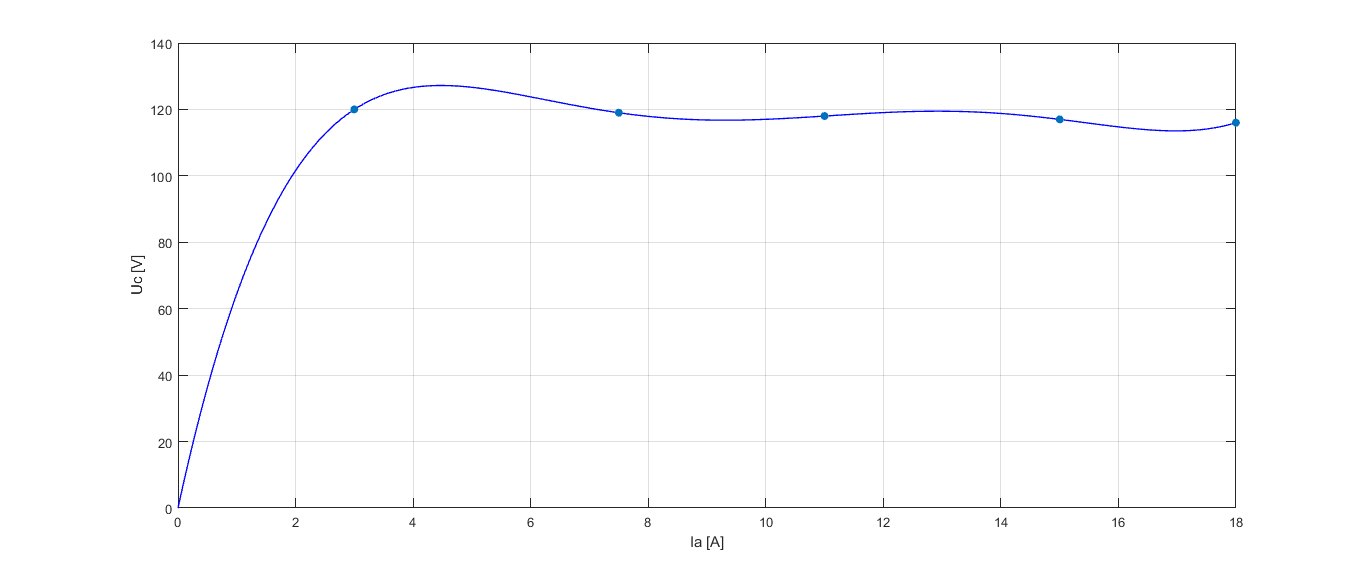
\includegraphics[scale=0.5]{./recursos-Lab6/CurvaDeCarga.png}
	\caption{Curva de carga experimental}
	\label{fig:CurvaDeCarga}
\end{figure}
\subsection{Características externas (Funcionamiento como motor)}
\subsubsection{Curva de velocidad respecto a la corriente de armadura}
	Se realiza la medición de la velocidad y la corriente de armadura empleando un rshunt, variando la carga y manteniendo fija la corriente de campo en 1,4 $\pm0,1$ A y la tensión nominal en 115V $\pm1$.\\
	
		La rshunt utilizada es de 40A@60mV, los valores de tensión obtenidos al estar en la escala de mV se multiplican por un factor de 4/6 para obtener la corriente que por ella circula.\\
		
		Sabemos que:
		
		\begin{equation}
			\tau_{ind}\cdot W_m = E_a*I_a 
			\label{ec.power}
		\end{equation}
		
		En la Figura \ref{fig:modObtenido} tenemos los parámetros internos obtenidos previamente, Al despejar $\tau_{ind}$ de la ecuación \ref{ec.power} y encontrando el valor de Ea obtenemos:
		
		\begin{equation}
			\tau_{ind}=\frac{U_n\cdot I_a-I_a^2\cdot R_a}{W_m}
		\end{equation}
		
		\begin{equation}
		\Delta \tau_{ind}=	\frac{\Delta Wn {\left({Ia}^2  Ra-Ia Un\right)}}{Wn^{2}}+\frac{Ia \Delta Un}{Wn}+\frac{ \Delta Ia {\left({Un}-2 {Ia} {Ra}\right)}}{{Wn}}+\frac{{Ia}^2 {\Delta Ra}}{Wn}
		\end{equation}
		
		Con las ecuaciones planteadas y datos obtenidos en el laboratorio se presenta el siguiente cuadro:
	\begin{table}[H]
		\centering
			\caption{Mediciones del efecto de la carga en la tensión del motor y medición indirecta de la corriente de armadura}
			\label{Cuadro valores de motor Iext ctte}
		\begin{tabular}{|c|c|c|c|c|}
			\hline
			Vshunt (mV) & N(rpm) & Carga (W) &Ia(A)& Tind\\ \hline
			11,8 $\pm$ 0,1 & 1010 $\pm$ 2 & 200 & 7,87 $\pm$ 0,07&8,39 $\pm$ 0,12\\ \hline
			13,5 $\pm$ 0,1 & 1008 $\pm$ 2 & 400 & 9,00 $\pm$ 0,07&9,58$\pm$0,13\\ \hline
			15,8 $\pm$ 0,1 & 1004 $\pm$ 2 & 600 & 10,53 $\pm$ 0,07&11,2$\pm$0,14\\ \hline
			17,0 $\pm$ 0,1 & 992 $\pm$ 2 & 800 & 11,33 $\pm$ 0,07& 12,20$\pm$0,15\\ \hline
			18,5$\pm$0,1 & 988$\pm$2 & 1000 & 12,33 $\pm$ 0,07& 13,30$\pm$1,15\\ \hline
			26,4$\pm$0,1 & 974$\pm$2 & 2000 & 17,60 $\pm$ 0,07&19,00$\pm$0,18\\ \hline
			28,2$\pm$0,1 & 968$\pm$2 & 2200 & 18,80 $\pm$ 0,07&20,30$\pm$0,19\\ \hline
		\end{tabular}
	\end{table}
Utilizando los datos obtenidos en el cuadro previo se graficó la curva deseada en la siguiente Figura.
	\begin{figure}[H]
	\centering
	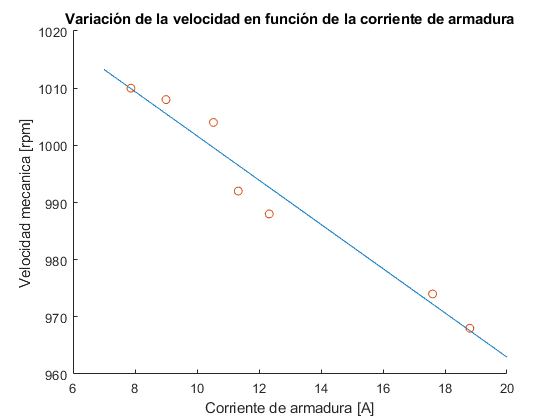
\includegraphics[scale=0.8]{./recursos-Lab6/curvaVelocidadCorriente.png}
	\caption{Curva a través de datos experimentales; velocidad en función de la corriente de armadura}
	\label{fig:CurvaDeVelocidadCorriente}
\end{figure}
	\begin{itemize}
		\item \textbf{Predeterminación de curva N=f(Ia)}
	\end{itemize}
	Para predeterminar la curva de velocidad con respecto a la corriente de armadura con $I_{ext}$ y $V_{T}$ constante se tiene la siguiente ecuación:
	\begin{equation}
		Ea= V_T - I_a * R_a = K \Phi N = AN
	\end{equation}
	En vacío se asumen las condiciones Ea = Vt =115, Ia=0 y N= 1000 rpm con lo que se contiene:
	\begin{equation}
		A=\frac{Ea}{N}= \frac{115}{1000}=0,115
		\label{ecuacion A}
	\end{equation}
	Con el valor de Ra previamente calculado es decir Ra= 0,2936 y la siguiente ecuación se predetermina la curva:
	\begin{equation}
	N =\frac{V_T - I_a * R_a}{A}
		\label{ec.Velocidad corriente}
	\end{equation}
		\begin{figure}[H]
		\centering
		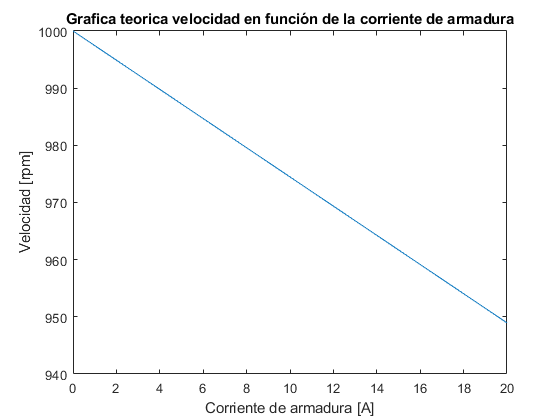
\includegraphics[scale=0.8]{./recursos-Lab6/curvaPredeterminarVelocidadCorrienteArmadura.png}
		\caption{Curva teórica de velocidad en función de la corriente de armadura}
		\label{fig:CurvaPredeterminarVelocidadCorrienteArmadura}
	\end{figure}
\subsubsection{Porcentaje de regulación de velocidad}
En el siguiente cuadro se observan la mediciones necesarias para obtener el porcentaje de regulación.
	\begin{table}[H]
		\centering
		\caption{Mediciones para el porcentaje de regulación}
		\label{Cuadro:Medicion porcentaje de regulacion}
		\begin{tabular}{|c|c|c|}
			\hline
			& pc & sc\\ \hline
			Vshunt(mV)& 32,0 $\pm$ 0,1 & 9,7 $\pm$ 0,1 \\ \hline
			$N$ (rpm)& 958 $\pm$ 2 &1040 $\pm$ 2 \\ \hline
			carga(KW)  & 2,8 &0\\ \hline
		\end{tabular}
	\end{table}

 Para determinar el porcentaje de regulación de velocidad se toman los datos del Cuadro \ref{Cuadro:Medicion porcentaje de regulacion} y a través de la siguientes formulas se determina el mismo.
 \begin{eqnarray}
  PRN_{\%} =100\%*\frac{n_{sc}-n_{pc}}{n_{pc}}; 
  & \Delta PNR = \frac{1 }{n_{pc}}\cdot \Delta n_{sc}+\frac{n_{sc} }{n_{pc}^2}\cdot \Delta n_{pc}
 \end{eqnarray}
 
De modo que el porcentaje de regulación de velocidad es de $8,56 \pm 0,0179 \%$
\begin{itemize}
	\item \textbf{Predeterminación de porcentaje de regulación}
\end{itemize}
En la siguiente expresión se observa el porcentaje de regulación teórico, calculado a partir de la ecuación \ref{ec.Velocidad corriente}, con $I_{a}$ a plena carga 26 A, $V_{T}$ 115 V y Ra 0,2936 $\Omega$.
\begin{equation}
\% PNR = \frac{N_{sc} - N {pc}}{N_{pc}} \cdot 100 \% = 7,10 \%
\end{equation}
\subsubsection{Curva de par en función de corriente armadura}
Utilizando los valores obtenidos en el cuadro \ref{Cuadro valores de motor Iext ctte} se graficó el par en función de la corriente en la siguiente Figura.
	\begin{figure}[H]
	\centering
	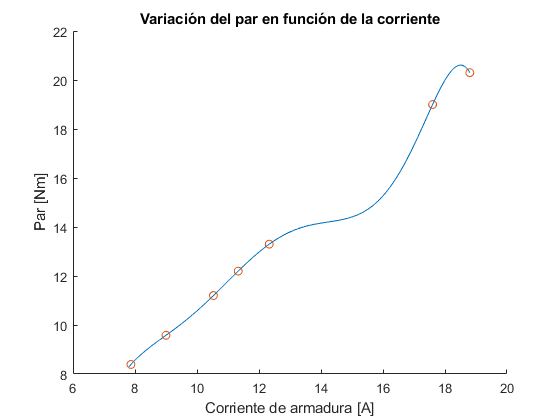
\includegraphics[scale=0.8]{./recursos-Lab6/curvaParCorrienteDeArmadura.png}
	\caption{Curva experimental de par en función de la corriente de armadura}
	\label{fig:CurvaDeParCorriente}
\end{figure}
\begin{itemize}
	\item \textbf{Predeterminación de la curva de par en función de la corriente de armadura}
\end{itemize}
Partiendo  de la siguiente expresión:
	\begin{equation}
		\tau = K \cdot \Phi \cdot Ia = A \cdot Ia
		\label{ecuacion par}
	\end{equation}
	
	El valor de $k\cdot \Phi$ se toma de la ecuación \ref{ecuacion A} 
	\begin{figure}[H]
	\centering
	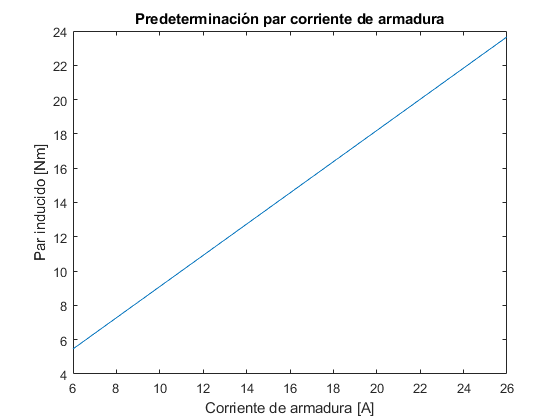
\includegraphics[scale=0.8]{./recursos-Lab6/curvaPredeterminarParCorrienteArmadura.png}
	\caption{Curva predeterminada de par en función de la corriente de armadura}
	\label{fig:CurvaPredeterminarDeParCorriente}
\end{figure}
\subsubsection{Curva de par en función de la velocidad}
Utilizando los valores obtenidos en el cuadro \ref{Cuadro valores de motor Iext ctte} se graficó la Figura \ref{fig:CurvaDeParVelocidad}.
	\begin{figure}[H]
	\centering
	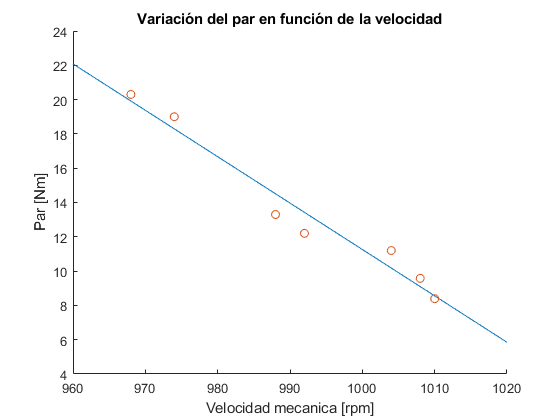
\includegraphics[scale=0.8]{./recursos-Lab6/curvaParVelocidad.png}
	\caption{Curva de par en función de la corriente de armadura}
	\label{fig:CurvaDeParVelocidad}
\end{figure}
	\begin{itemize}
	\item \textbf{Predeterminación de curva de par en función de la Velocidad}
\end{itemize}
Para predeterminar el par en función de la velocidad de salida se parte de las ecuaciones \ref{ec.Velocidad corriente} y \ref{ecuacion par} dando como resultado:
\begin{eqnarray}
\tau = \frac{A}{R_a}\cdot (Vt- N \cdot A)
\end{eqnarray}

\begin{figure}[H]
	\centering
	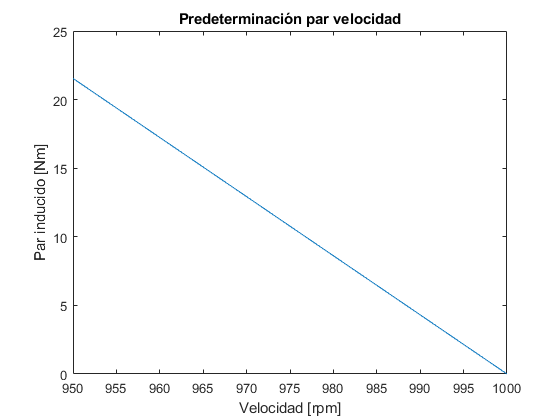
\includegraphics[scale=0.8]{./recursos-Lab6/curvaPredeterminarParVelocidad.png}
	\caption{Curva de par en función de la corriente de armadura}
	\label{fig:CurvapredeterminadaDeParVelocidad}
\end{figure}
\subsubsection{Curva de velocidad en función de la tensión de entrada}
Unicamente se realizo la predeterminación, ya que en la boratorio no se ajusto la tensión con el fin de observar el efecto en la velocidad del motor, dicha curva se encuentra en la Figura \ref{fig:curvaPredeterminadaVelocidadTension}.
\begin{figure}[H]
	\centering
	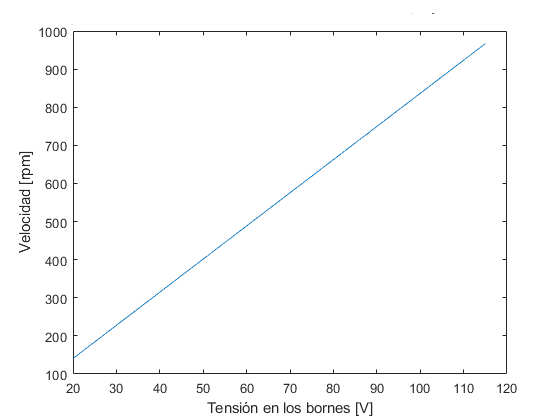
\includegraphics[scale=0.8]{./recursos-Lab6/curvaPredeterminarVelocidadTension.png}
	\caption{Curva de par en función de la corriente de armadura}
	\label{fig:curvaPredeterminadaVelocidadTension}
\end{figure}

\subsubsection{Medición de pérdidas en vacío}
Se realizaron las siguientes mediciones:
\begin{table}[H]
	\centering
	\caption{Pruebas de medición de perdidas en vacío}
	\begin{tabular}{|c|c|c|c|c|}
		\hline
	Medición	& $V_t$ [V] & N [rpm] & Vshunt [mV] & $I_a$ [A] \\ \hline
	1 & 120 $\pm$1& 1040 $\pm$ 2 & 8,3 $\pm$0,1 & 5,53 $\pm$ 0,066 \\ \hline 
	2 & 120 $\pm$1& 1252 $\pm$ 2 & 9,7 $\pm$0,1 & 6,47 $\pm$ 0,066\\ \hline
	\end{tabular}
\end{table}
Para el calculo de las pérdidas en vacío se emplean las siguientes ecuaciones:
\begin{eqnarray}
Po1 = K_f N1 E1  + Kh N1^2E1^2\\
Po2 = K_f N2 E1  + Kh N2^2E1^2
\end{eqnarray}

Para los correctos cálculos se requerían de 4 mediciones, debido a que se tomaron 2 no es posible calcular las perdidas en vacío. En consecuencia sin las perdidas no es posible hallar la la eficiencia de la maquina.


\section{Análisis de resultados}
\subsection{Características internas}
Se comprobó que efectivamente la resistencia de campo es varias veces más grande que la serie y la de armadura, por otro lado el efecto de la temperatura es lo suficientemente grande como para ser imposible el ignorarlo, al momento de ajustar las resistencias a los valores usados en el modelo\\

En la prueba de vacío al ajustar la curva mediante mínimos cuadrados, se observa cierta deformación en la curva descendente de vacío, esto se debe unicamente a que se rompio la equidistancia entre dos mediciones adyacentes, no se regreso ajustando al valor adecuado debido a que el ciclo de histeresis obtenido sería erroneo. El motivo por el cual la curva descendente se encuentra por encima de la ascendente es debido a que existe un flujo remanente, dicho flujo solo puede ser eliminado con una fuerza coercitiva en la dirección adecuada. Al comparar el ciclo con el del transformador se observa que las perdidas por histeresis son menores, por supuesto esto dependerá de la construcción de la maquina DC y el transformador a comparar.
\subsection{Características Externas (Funcionando como generador)}
Al hallar la curva de regulación en la Figura \ref{fig:curvaCaractReg} se observa el efecto de la reacción de armadura en la corriente de excitación, ya que a pesar de ser leve existe, para que no existiese, la corriente de excitación debería mantenerse constante respecto a las variaciones en la carga. Cabe destacar que en la Figura \ref{fig:curvaDeRegComparacion}, se observa como si la curva experimental fuese muy distinta a la obtenida mediante el calculo, aunque la realidad es que la calculada  siempre se encuentra dentro de la incertidumbre de las mediciones realizadas, también es necesario tomar en cuenta que la curva calculada se tomo para un $N_{f}$ arbitrario. Dados los resultados, el valor real debe encontrarse cerca de las 1000 vueltas. 

En el caso de la curva de carga se observa que al colocar distintas cargas, estas afectaran al flujo haciéndolo cada vez mayor, de igual forma al aumentar la corriente el efecto de la resistencia de armadura se hará cada vez más notable, de modo que siempre tendera a decaer la tensión en los bornes porque a pesar de que $E_{a}$ aumenta por el flujo y esto se contrapone con la caída en la resistencia, el flujo de toda máquina tiene un limite en el cual se satura, mientras que la corriente no. Y dado que los motores DC suelen trabajarse en el codo de saturación dicho limite se encuentra bastante cerca del punto de trabajo, de modo que el decaimiento en la tensión es visible a medida que se aumenta la carga. Por supuesto dicho decaimiento se le conoce como regulación, esta fue calculada en (5,6 $\pm$ 0,8) \%.
\subsection{Características Externas (Funcionando como motor)}
En la Figura \ref{fig:CurvaDeVelocidadCorriente} se observa la curva de velocidad en función de la corriente de armadura, segun la predeterminación esta debería se una recta sin embargo varios de los puntos se alejan del comportamiento deseado más de lo que deberían, esto se debe a que al ajustar el campo, para obtener tensión nominal, la corriente en el mismo se alejaba en cierta medida de su valor de excitación en vacío, por lo que se observa un leve efecto de reacción de armadura al final de la curva, sin embargo los resultados son adecuados a la forma en la que se midió.

El porcentaje de regulación es ligeramente superior al valor esperado en las predeterminaciones, esto puede deberse a que al calcular teóricamente no se esta tomando en cuenta las perdidas mecánicas, del generador acoplado al motor. Sin embargo el que la regulación sea superior al valor esperado es un valor satisfactorio.

En la curva de par corriente de armadura se observa un comportamiento bastante lineal y parecido a su predeterminación y como es de esperarse a medida que aumenta la carga el par incrementara.

La curva de par velocidad se encuentra sujeta a incertidumbres mayores que la previa, debido a que esta fue determinada utilizando dos mediciones que no es posible medirlas directamente en el laboratorio. No obstante se obtuvo un comportamiento similar a su predeterminación. 
\newpage 
  \section{Conclusión}
  El caracterizar una maquina DC es una tarea repetitiva que requiere múltiples mediciones para conocer su comportamiento. Las características internas son comunes para cualquier conexión que se le aplique a la maquina, pero las externas dependen del tipo de conexión, ya que modifican el comportamiento de la maquina por completo, por supuesto existen similitudes. Las ecuaciones que rigen a cada modelo son completamente distintas, e incluso aunque en papel un generador y un motor con la misma conexión posean el mismo comportamiento con la diferencia de la dirección de la energía en la realidad una maquina funcionando como motor puede tener o no los mismos valores nominales,esto modifica completamente la forma en la que se realizaran las conexiones de la maquina, puesto que por ejemplo el hecho de tener corrientes distintas implica un cambio en el diámetro de los conductores.
  
  En definitiva si se quiere obtener un modelo de la maquina ajustado a lo que refiere el fabricante es necesario cumplir fielmente las condiciones impuestas en la norma IEEEE-113 
\newpage
  \section{Anexos}
  	\begin{figure}[H]
  	\centering
  	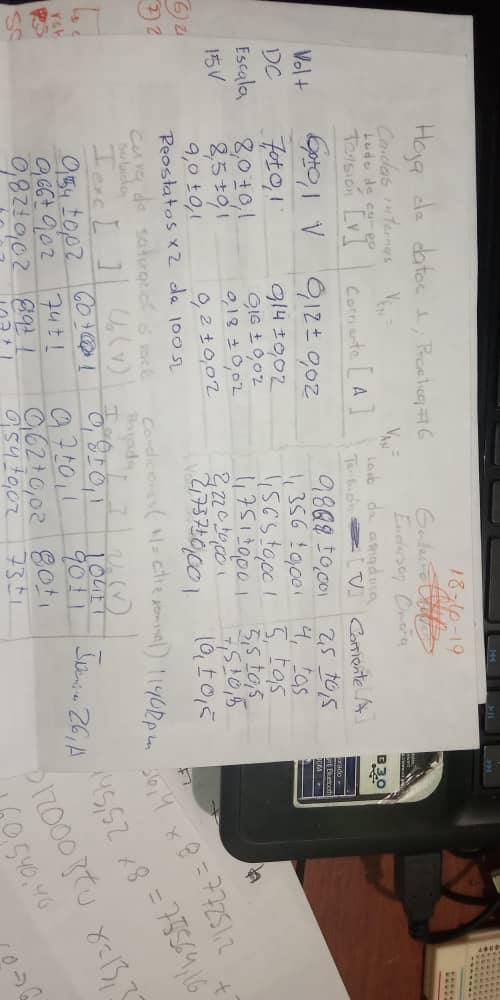
\includegraphics[scale=0.8]{./recursos-Lab6/HojaDeDatosA.jpeg}
  	\caption{Hoja de datos parte A}
  	\label{fig:Hoja1}
  	\end{figure}  
  \begin{figure}[H]
  	\centering
  	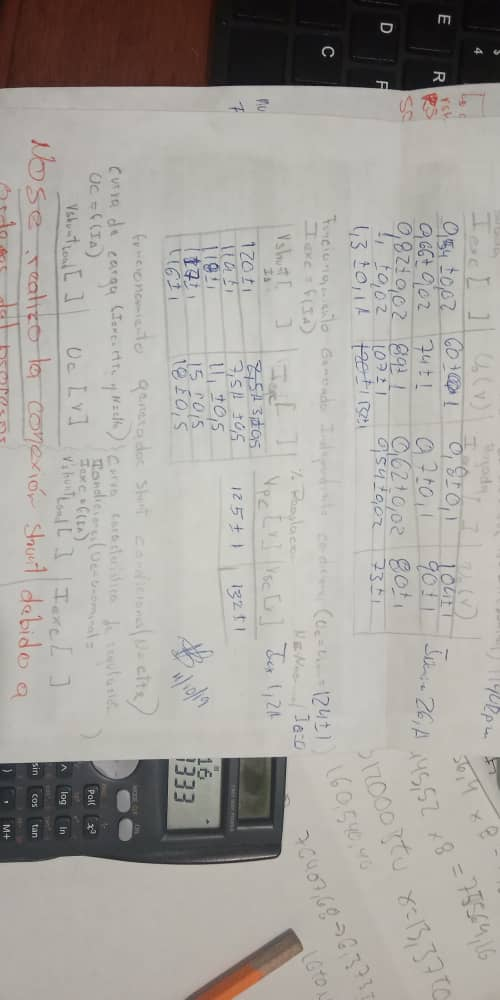
\includegraphics[scale=0.8]{./recursos-Lab6/HojaDeDatosB.jpeg}
  	\caption{Hoja de datos parte B}
  	\label{fig:Hoja2}
  \end{figure}
\begin{figure}[H]
	\centering
	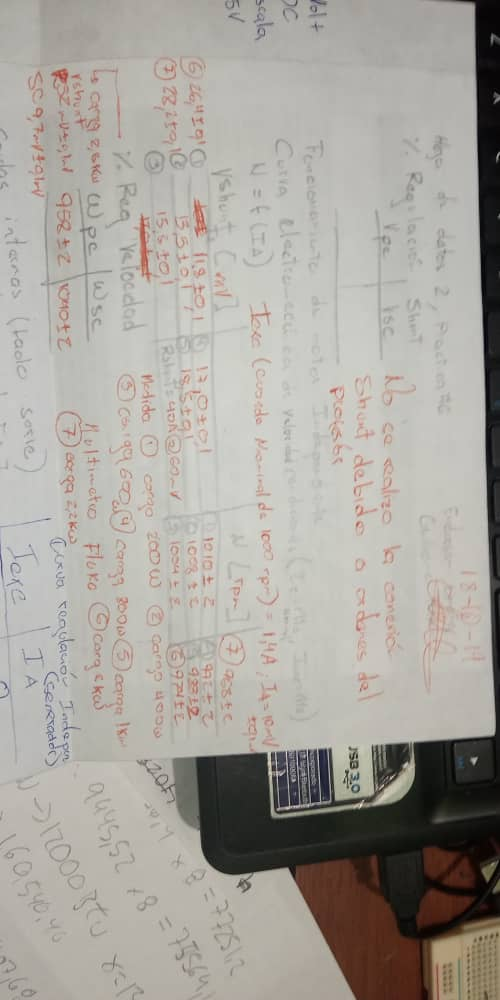
\includegraphics[scale=0.6]{./recursos-Lab6/HojaDeDatosC.jpeg}
	\caption{Hoja de datos parte C}
	\label{fig:Hoja3}
\end{figure}
\begin{figure}[H]
	\centering
	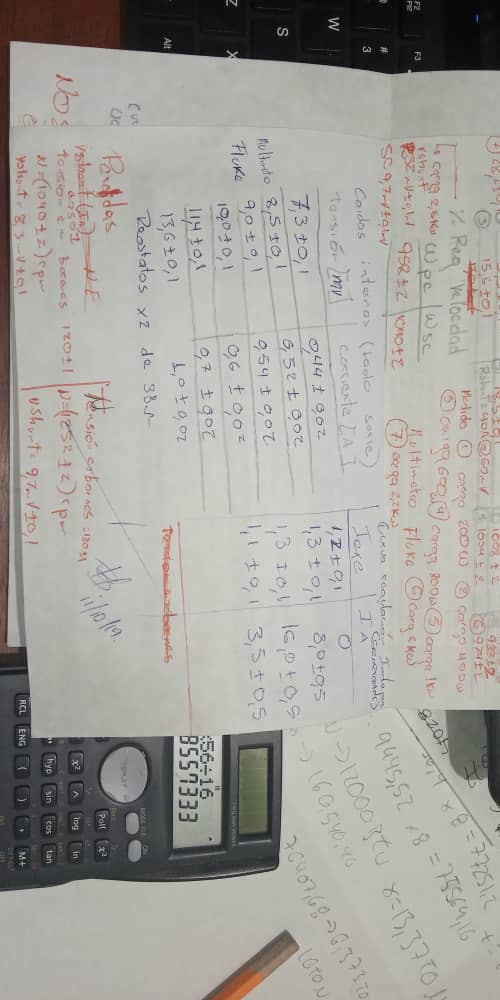
\includegraphics[scale=0.8]{./recursos-Lab6/HojaDeDatosD.jpeg}
	\caption{Hoja de datos parte D}
	\label{fig:Hoja4}
\end{figure}
\end{document}
